\documentclass{article}
\usepackage{polski}
\usepackage[utf8]{inputenc}
\usepackage{hyperref}
\usepackage{graphicx}
\graphicspath{ {./} }

\title{Redmine, issue tracker}
\author{Marcin Kostrzewski, 444409}
\date{13 Września, 2019r}

\begin{document}

\maketitle
\newpage

\section{Wprowadzenie}
\textbf{Redmine} to narzędzie typu issue tracker oparte na bazie licencji
\textit{GNU}, czyli jest całkowicie darmowe. Mamy również bezpośredni
dostęp do jego kodu źródłowego. Program został napisany na frameworu
\textit{Ruby on Rails} i jest wieloplatformowy. Redmine powstał w czerwcu 2006 roku, czyli
system ma już 13 lat. Korzystają z niego takie systemy jak \textit{FreeNAS}, język \textit{Ruby}, \textit{Alpine Linux}.

\section{Instalacja}
Instalacja całego systemu jest dosyć skomplikowana i wymaga wielu
zewnętrznych programów i systemów. Oprócz samych plików instalacyjnych
Redmine, będziemy potrzebować:
\begin{itemize}
    \item \textit{Interpreter Ruby}
    \item \textit{Back-end bazy danych, np MySQL}
\end{itemize}
Następnie musimy skonfigurować bazę danych, zainstalować dependencje,
ustawić odpowiednie uprawnienia. Cały proces jest całkiem skomplikowany
i czasochłonny, na szczęście Redmine oferuje użytkownikowi dostęp do 
publicznego wiki, na którym cały proces instalacji i konfiguracji jest
dokładnie opisany. Możemy go znaleźć tutaj: \url{https://www.redmine.org/projects/redmine/wiki/RedmineInstall}

\section{Wersja demo}
Redmine oferuje dostęp do tzw. wersji demonstracyjnej programu
dostępnej z poziomu przeglądarki. Jest to bardzo dobra opcja
w przypadku, gdy chcemy zobaczyć jak działa cały system bez
przechodzenia przez czasochłonny proces instalacji.
Demo dostępne jest pod adresem \url{http://demo.redmine.org}

\section{Zakładanie konta i tworzenie projektu}
\textit{Proces ten omówię na podstawie wersji demo. Dla własnych
instalacji, proces wygląda identycznie.}
\newpage
\subsection{Tworzenie konta}
W prawym górnym rogu znajdują się dwa małe przyciski: \textit{Sign in} i \textit{Register}.
Klikamy w ten drugi i wypełniamy formularz rejestracyjny.
\begin{center}
    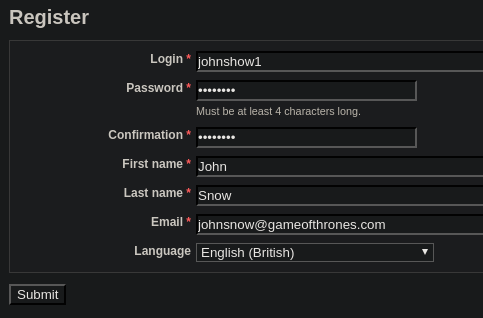
\includegraphics[scale=0.6]{register.png}
\end{center}
Po wysłaniu formularza powinniśmy potwierdzić naszą rejestrację
otwierając naszego maila i klikając w link aktywacyjny. \textit{
    Na wersji demo nie musimy tego robić, nasze konto zostanie
    automatycznie aktywowane.
}

\subsection{Zakładanie nowego projektu}
W górnym pasku, po lewej stronie wchodzimy w zakładkę \textit{Projects}
a następnie klikamy na przycisk 
\includegraphics[]{newproject.png}.
Zostaniemy przekierowani do formularza nowego projektu.
\begin{center}
    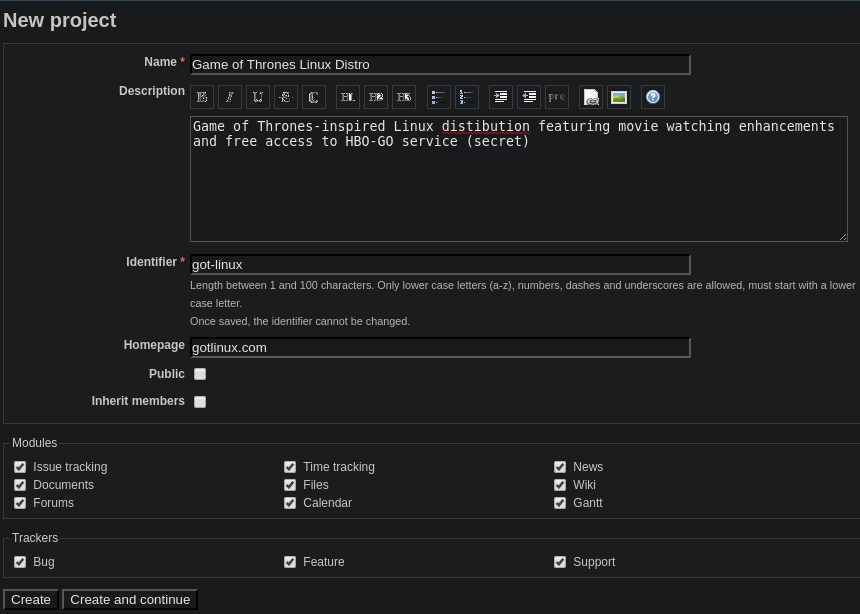
\includegraphics[scale=0.4]{projectform.png}
\end{center} 
Możemy wybrać jakie moduły będą zawarte w naszym projekcie, np \textit{Wiki}, \textit{Forums}, itp.
\newline
Tworzymy projekt i wracamy do zakładki z projektami. Powinniśmy znaleźć
tam nasz nowo stworzony projekt.
\begin{center}
    
\includegraphics[scale=0.5]{myproject.png}
\end{center}

\subsection{Zarządzanie projektem}
\begin{center}
    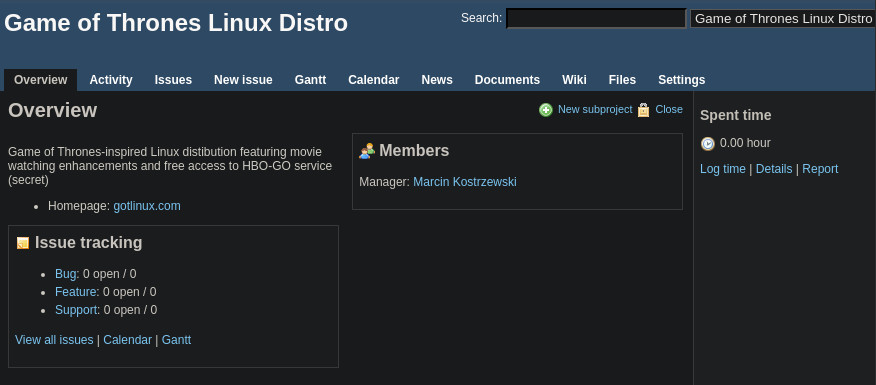
\includegraphics[scale=0.5]{dashboard.png}
\end{center}
Jak widzimy, panel projektu oferuje nam sporo możliwości.
Z tego miejsca możemy zarządzać wszystkimi działami naszego projektu,
mamy tutaj dostęp do modyfikacji wiki, możemy tworzyć nowe zadania,
zarządzać kalendarzem, załączać dokumenty i pliki.

\section{Kilka słów kończoncych}
Po skorzystaniu z Redmine byłem bardzo zaskoczony prostotą i przejrzystością
interfejsu. Mimo wielu licznych opcji, nie był on tak przeładowany
i skomplikowany jak np. interfejs Jiry, na której pracujemy na 
zajęciach. Ciekawym modułem jesst Wiki, gdzie możemy tworzyć
np. dokumentacje, która ujrzy światło dzienne. Oprócz tego
obsługa kalendarza jest dziecinnie prosta, mimo wielu
funkcji. Program może jednak wyglądać nieco archaicznie, ale 
w internecie możemy znaleźć wiele modyfikacji poprawiająych
frontend aplikacji. Myślę, że mógłbym skorzystać z Redmine tworząc
np. projekt inżynierski.
\end{document}